\documentclass[12pt]{article}

\usepackage{fullpage}
\usepackage{graphicx}
\usepackage{amssymb}
\usepackage{amsmath}
\usepackage[none]{hyphenat}
\usepackage{parskip}
\usepackage[spanish]{babel}
\usepackage[utf8]{inputenc}
\usepackage{hyperref}
\usepackage{fancyhdr}
\usepackage{tasks}
\usepackage{mdframed}
\usepackage{xcolor}
\usepackage{pgfplots}
\usepackage[makeroom]{cancel}
\usepackage{multicol}
\usepackage[shortlabels]{enumitem}
\usepackage{stackrel}
\usepackage{tkz-tab}
\usepackage{xpatch}
\usepackage{tkz-euclide}
\usetkzobj{all}
\xpatchcmd{\tkzTabLine}{$0$}{$\bullet$}{}{}

\setlength{\headheight}{10pt}
\setlength{\headsep}{10pt}
\pagestyle{fancy}
\rhead{\ayudantia \ - \alumno}
\tikzset{t style/.style={style=solid}}

\newcommand*{\mybox}[2]{\colorbox{#1!30}{\parbox{.98\linewidth}{#2}}}

\newenvironment{solucion}
{\begin{mdframed}[backgroundcolor=black!10]
		{\bf Solución:}\\
	}
	{
	\end{mdframed}
}

\newenvironment{alternativas}[1]
{\begin{multicols}{#1}
		\begin{enumerate}[a)]
		}
		{
		\end{enumerate}
	\end{multicols}
}

\newenvironment{preguntas}
{\begin{enumerate}\itemsep12pt
	}
	{
	\end{enumerate}
}

\newcommand{\ayudantia}{{\sc Ayudantía 3}}
\newcommand{\tituloayu}{Series I}
\newcommand{\fecha}{27 de agosto de 2019}
\newcommand{\sigla}{MAT1620}
\newcommand{\nombre}{Cálculo II}
\newcommand{\profesor}{Wolfgang Rivera}
\newcommand{\ano}{2019}
\newcommand{\semestre}{2}
\newcommand{\mail}{mat1620@ifcastaneda.cl}
\newcommand{\alumno}{Ignacio Castañeda - \mail}

\newcommand{\ev}{\Big|}
\newcommand{\ra}{\rightarrow}
\newcommand{\lra}{\leftrightarrow}
\newcommand{\N}{\mathbb{N}}
\newcommand{\R}{\mathbb{R}}
\newcommand{\Exp}[1]{\mathcal{E}_{#1}}
\newcommand{\List}[1]{\mathcal{L}_{#1}}
\newcommand{\EN}{\Exp{\N}}
\newcommand{\LN}{\List{\N}}
\newcommand{\comment}[1]{}
\newcommand{\lb}{\\~\\}
\newcommand{\eop}{_{\square}}
\newcommand{\hsig}{\hat{\sigma}}
\newcommand{\widesim}[2][1.5]{
	\mathrel{\overset{#2}{\scalebox{#1}[1]{$\sim$}}}
}
\newcommand{\wsim}{\widesim{}}
\newcommand{\lh}{\stackrel{L'H}{=}}

\begin{document}
\thispagestyle{empty}

\begin{minipage}{2cm}
	
\includegraphics[width=2cm]{../../../../img/logo.pdf}
	\vspace{0.5cm}
\end{minipage}
\begin{minipage}{\linewidth}
	\begin{tabular}{lrl}
		{\scriptsize\sc Pontificia Universidad Catolica de Chile} & \hspace*{0.7in}Curso: &
		\sigla  - \nombre\\
		{\sc Facultad de Matemáticas}&
		Profesor: & \profesor \\
		{\sc Semestre \ano-\semestre} & Ayudante: & {Ignacio Castañeda}\\
		& {Mail:} & \texttt{\mail}
	\end{tabular}
\end{minipage}

\vspace{-10mm}
\begin{center}
	{\LARGE\bf \ayudantia}\\
	\vspace{0.1cm}
	{\tituloayu}\\
	\vspace{0.1cm}
	\fecha\\
	\vspace{0.4cm}
\end{center}

\begin{preguntas}
\item Determine si las siguientes series convergen o divergen.
\begin{tasks}(3)
\task $\sum\limits_{n=1}^{\infty}\dfrac{5n^3}{7n+n^3-1}$
\task $\sum\limits_{n=1}^{\infty}\left(sen\left(\dfrac{n\pi}{2}\right)\right)^2$
\task $\sum\limits_{n=1}^{\infty}2^{2n}3^{1-3n}$
\task $\sum\limits_{n=1}^{\infty}\dfrac{1 + n + \sin(n)}{3n^4 + \ln(n)}$
\task $\sum\limits_{n=20}^{\infty}\dfrac{1}{nln(n)ln(ln(n))}$
\task $\sum\limits_{n=1}^{\infty}ln\left(1+\dfrac{1}{n}\right)$
\end{tasks}
\begin{solucion}
\begin{center}
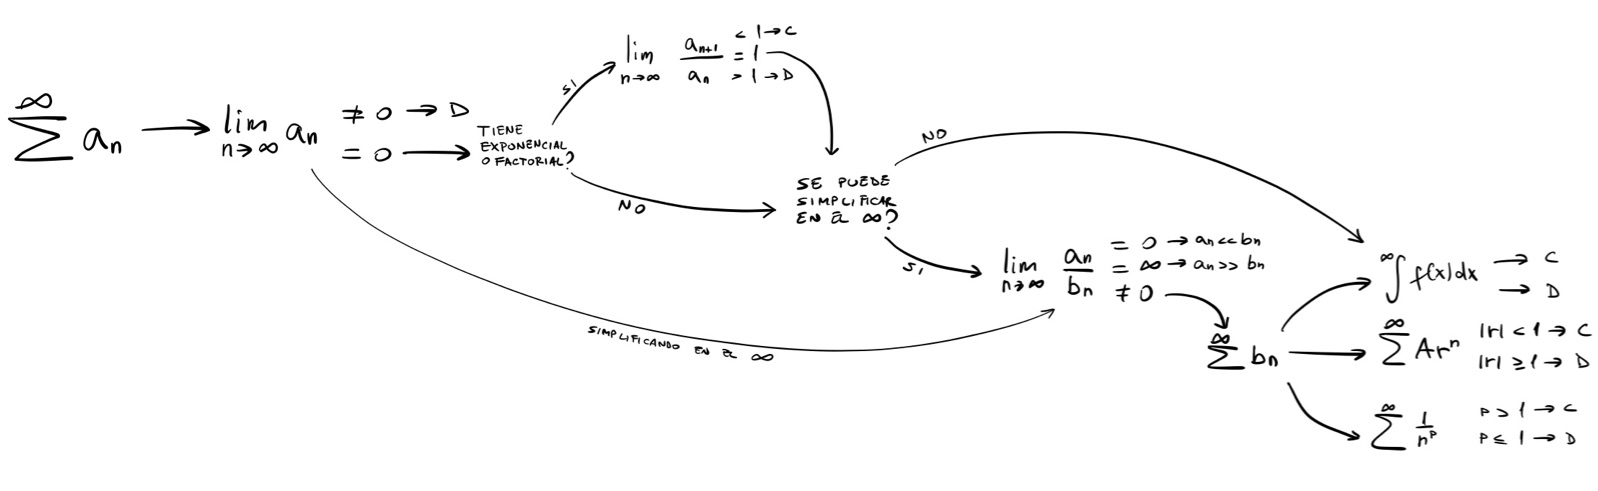
\includegraphics[width=8cm]{../../../../img/mapa_series}
\end{center}
\begin{enumerate}[a)]
\item $\sum\limits_{n=1}^{\infty}\dfrac{5n^3}{7n+n^3-1}$\\
			\\
			En primer lugar, veamos el límite de la sucesión, esto es
			$$\lim\limits_{n\ra \infty} \dfrac{5n^3}{7n+n^3-1} = 5 \neq 0$$
			Entonces, por la prueba de la divergencia, concluimos que la serie diverge.
\item $\sum\limits_{n=1}^{\infty}\left(sen\left(\dfrac{n\pi}{2}\right)\right)^2$\\
			\\
			Veamos el límite de la sucesión
			$$\lim\limits_{n\ra \infty} \left(sen\left(\dfrac{n\pi}{2}\right)\right)^2 \ra alternante \neq 0$$
			Por la prueba de la divergencia, la serie diverge.
\item $\sum\limits_{n=1}^{\infty}2^{2n}3^{1-3n}$\\
			\\
			Notemos que esta es una serie geométrica, por lo que debemos escribirla de la forma $\sum\limits_1^{\infty} Ar^n$ para saber como se comporta.
$$\sum\limits_{n=1}^{\infty}2^{2n}3^{1-3n} 
= \sum\limits_{n=1}^{\infty}2^{2n} \dfrac{3}{3^{3n}}
= \sum\limits_{n=1}^{\infty}(2^2)^n \dfrac{3}{(3^3)^n}
= \sum\limits_{n=1}^{\infty}4^n \dfrac{3}{27^n}
= \sum\limits_{n=1}^{\infty} 3 \left(\dfrac{4}{27}\right)^n$$
			Como $r = \dfrac{4}{27} <1$, la serie converge.
\item $\sum\limits_{n=1}^{\infty}\dfrac{1 + n + \sin(n)}{3n^4 + \ln(n)}$\\
			\\
En primer lugar, notemos que
$$\lim\limits_{n\ra \infty} \dfrac{1 + n + \sin(n)}{3n^4 + \ln(n)}
= \lim\limits_{n\ra \infty} \dfrac{n\left(\cancelto{0}{\frac{1}{n}} + 1 + \cancelto{0}{\frac{\sin(n)}{n}}\right)}{n^4\left(3 + \cancelto{0}{\frac{\ln(n)}{n^4}}\right)}
= \lim\limits_{n\ra \infty} \dfrac{n}{3n^4}
= \lim\limits_{n\ra \infty} \dfrac{1}{3n^3} = 0$$
Luego, usando $b_n = \dfrac{1}{3n^3}$, se cumple que
$$\lim\limits_{n\ra \infty} \dfrac{\dfrac{1 + n + \sin(n)}{3n^4 + \ln(n)}}{\dfrac{1}{3n^3}}
= \lim\limits_{n\ra \infty} \dfrac{\dfrac{1}{3n^3}}{\dfrac{1}{3n^3}} 
= 1 \neq 0$$
Notemos que $\sum\limits_{n=1}^{\infty} \dfrac{1}{3n^3}$ es es una $serie-p$ con $p=3>1$, por lo que la serie es convergente. Luego, por criterio de comparación al límite, $\sum\limits_{n=1}^{\infty}\dfrac{1 + n + \sin(n)}{3n^4 + \ln(n)}$ también converge.
\item $\sum\limits_{n=20}^{\infty}\dfrac{1}{nln(n)ln(ln(n))}$\\
			\\
			Sea
			$$a_n = \dfrac{1}{nln(n)ln(ln(n))} \ra f(x) = \dfrac{1}{xln(x)ln(ln(x))}$$
			Usando el criterio de la integral, $\displaystyle\int_{20}^{\infty}f(x)dx$ se comportará igual que $\sum\limits_{n=20}^{\infty} a_n$, por lo que debemos ver la convergencia de la integral en cuestión
			$$\int_{20}^{\infty} \dfrac{1}{xln(x)ln(ln(x))} dx$$
			Usando $u=ln(ln(x)) \ra du = \dfrac{dx}{xln(x)}$,
			$$\int_{20}^{\infty} \dfrac{1}{xln(x)ln(ln(x))} dx
			= \int_{ln(ln(20))}^{\infty} \dfrac{du}{u} = ln(u) \ev_{ln(ln(20))}^{\infty}$$
			$$ = ln(\infty) - ln(ln(ln(20))) = \infty = \not \exists$$
			Finalmente, por el criterio de la integral, la serie converge.
\item  $\sum\limits_{n=1}^{\infty}ln\left(1+\dfrac{1}{n}\right)$\\
			\\
			Notemos que
			$$\sum\limits_{n=1}^{\infty} ln\left(1+\dfrac{1}{n}\right)
			= \sum\limits_{n=1}^{\infty} ln\left(\dfrac{n+1}{n}\right)
			= \sum\limits_{n=1}^{\infty} ln(n+1)-ln(n)$$
			Es una serie telescopica. Expandiendo términos
			$$= (ln(2)-ln(1)) + (ln(3)-ln(2)) + \dots + (ln(n) - ln(n-1)) + (ln(n+1) - ln(n))$$
			$$= (\cancel{ln(2)}-ln(1)) + (\cancel{ln(3)}-\cancel{ln(2)}) + \cancel{\dots} + (\cancel{ln(n)} - \cancel{ln(n-1)}) + (ln(n+1) - \cancel{ln(n)})$$
			$$= ln(n+1) - ln(1)$$
			$$\lim\limits_{n \ra \infty} ln(n+1) = ln(\infty) = \infty = \not \exists$$
			Finalmente, la serie es divergente.
\end{enumerate}
\end{solucion}
\item Demuestre que si $\sum\limits_{n=1}^{\infty}a_n$ es convergente, entonces el limite de la sucesión $b_n=ln(1+a_n)$ en el infinito es $0$.
\begin{solucion}
Como $\sum\limits_{n=1}^{\infty}a_n$ es convergente, entonces debe ocurrir que
$\lim\limits_{x \ra \infty} a_n = 0$.\\

Luego,
$$\lim\limits_{x \ra \infty} b_n
= \lim\limits_{x \ra \infty} ln(1+a_n)
= ln(1+\lim\limits_{x \ra \infty} a_n)
= ln(1+0)
= 0$$

$$\blacksquare$$
\end{solucion}
\item Sea $a_n$ una sucesión tal que $a_n \neq 0,\ \forall n \in \N$.\\
	Demuestre que si $\sum\limits_{n=1}^{\infty}a_n$ converge, entonces $\sum\limits_{n=1}^{\infty}\dfrac{1}{a_n}$ diverge.
\begin{solucion}

\end{solucion}
\item Considere una función $f$ continua en $\R$, decreciente y no negativa tal que
	$$\lim_{x\ra\infty}\dfrac{f(x)}{e^{-x}}=5$$
	Analice la convergencia de la serie $\sum\limits_{n=1}^{\infty}f(n)$
\begin{solucion}
Sabemos que
		$$\lim_{x\ra\infty}\dfrac{f(x)}{e^{-x}}=5 \neq 0$$
		Por lo tanto, por el criterio de comparación al límite, $\sum\limits_{n=1}^{\infty}f(n)$ se comporta igual que $\sum\limits_{n=1}^{\infty}e^{-n}$\\
		\\
		Veamos la convergencia de 
		$$\sum\limits_{n=1}^{\infty}e^{-n}$$
		Usando el criterio de la razón,
		$$\lim\limits_{n \ra \infty} \dfrac{a_{n+1}}{a_n}
		= \lim\limits_{n \ra \infty} \dfrac{e^{-n-1}}{e^{-n}}
		= e^{-1} < 1$$
		Por lo tanto, es convergente. De la misma forma, la serie $\sum\limits_{n=1}^{\infty}f(n)$ también lo es.
\end{solucion}
\item Considere la representación decimal de un número,
$$0,d_1d_2d_3... = \dfrac{d_1}{10} + \dfrac{d_2}{10^2} + \dfrac{d_3}{10^3}$$
donde $d_i$ es alguno de los dígitos entre 0 y 9. Pruebe que la serie anterior es convergente.
\begin{solucion}

\end{solucion}
\end{preguntas}
\end{document}